\documentclass[tikz,border=10pt]{standalone}
\usepackage{tikz}
\usetikzlibrary{positioning}

% Global styles for nodes and paths
\tikzset{
  every node/.style={text=black, draw=black, font=\Large, line width=0.5mm},
  every path/.style={draw=black, line width=0.5mm}
}

\begin{document}
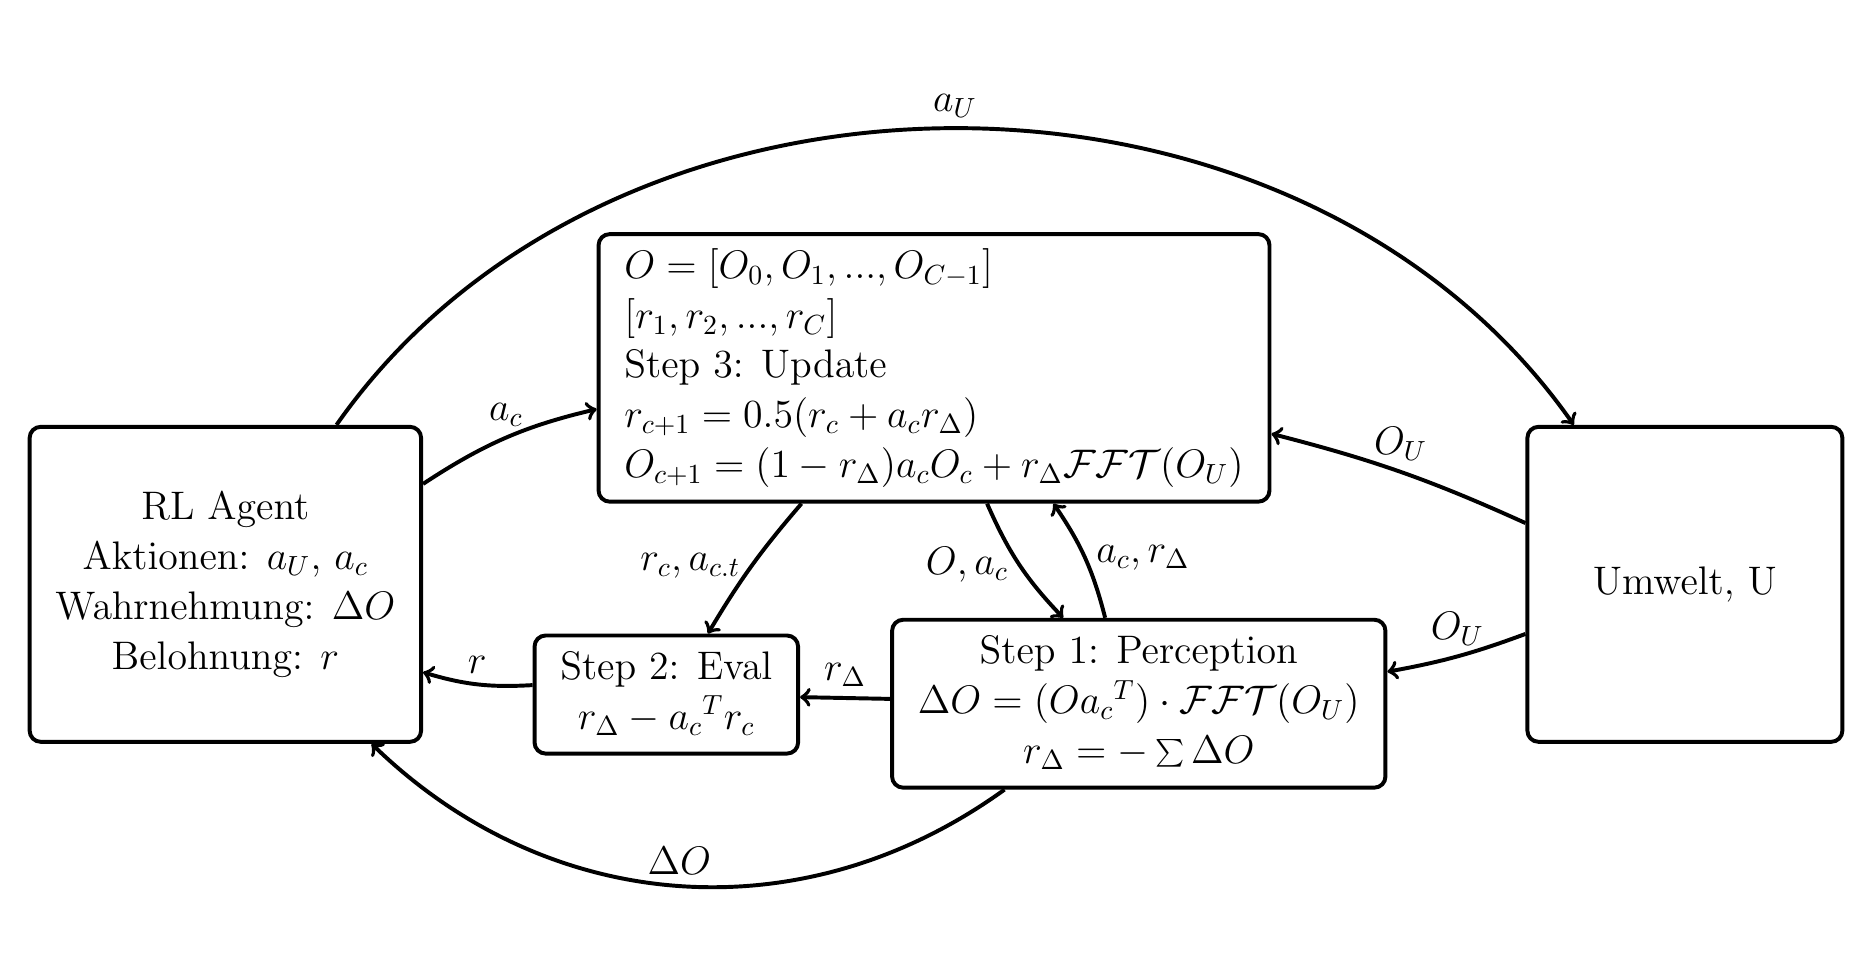
\begin{tikzpicture}[node distance=2cm, auto]
  % Nodes 
  \node (agent) [minimum width=4cm, minimum height=4cm, rounded corners] {
    \begin{tabular}{c}  
      RL Agent\\ 
      Aktionen: $a_U$, $a_c$ \\
      Wahrnehmung: $\Delta O$ \\
      Belohnung: $r$
    \end{tabular}
    };
  \node (memory) [above=-1cm of agent, xshift=9cm, minimum width=6cm, minimum height=2cm, rounded corners]  {
      \begin{tabular}{l}
      $ O = [O_0, O_1, ..., O_{C-1}] $ \\
      $ [r_1, r_2, ..., r_C] $\\
      Step 3: Update \\
      $ r_{c + 1} = 0.5(r_{c} + a_cr_{\Delta}) $ \\
      $ O_{c + 1} = (1 - r_{\Delta})a_{c}O_{c} + r_{\Delta}\mathcal{F} \mathcal{F} \mathcal{T} (O_{U}) $ 
      \end{tabular}
  };
  \node (world) [right=14cm of agent, minimum width=4cm, minimum height=4cm, rounded corners] {Umwelt, U};
  \node (evaluator) [rectangle, below=-1.4cm of agent, xshift=5.6cm, rounded corners] {
    \begin{tabular}{c}  Step 2: Eval \\ $r_{\Delta} - {{a_c}^T r_c}$ \end{tabular}
  };
  \node (calculator) [rectangle, below=-1.6cm of agent, xshift=11.6cm, rounded corners] {
    \begin{tabular}{c} 
      Step 1: Perception\\ 
      $\Delta O = (O {a_c}^T)\cdot \mathcal{F} \mathcal{F} \mathcal{T} (O_{U})$ \\
      $ r_{\Delta} = -\sum \Delta O$ \\
    \end{tabular}
  };

  \draw[->] (calculator) to[bend left=40] node[midway, above, draw=none, fill=none] {$\Delta O$} (agent);
  \draw[->] (memory) to[bend right=5] node[midway, left, draw=none, fill=none] {$r_{c}, a_{c. t}$} (evaluator);
  \draw[->] (world) to[bend left=5] node[midway, above, draw=none, fill=none] {$O_{U}$} (calculator);
  \draw[->] (memory) to[bend right=10] node[midway, left, draw=none, fill=none] {$O, a_c$} (calculator);
  \draw[->] (calculator) to[bend left=0] node[midway, above, draw=none, fill=none] {$r_{\Delta}$} (evaluator);
  \draw[->] (calculator) to[bend right=10] node[midway, right, draw=none, fill=none] {$a_c, r_{\Delta}$} (memory);
  \draw[->] (agent) to[bend left=10] node[midway, above, draw=none, fill=none] {$a_c$} (memory);
  \draw[->] (agent) to[bend left=55] node[midway, above, draw=none, fill=none] {$a_{U}$} (world);
  \draw[->] (world) to[bend right=5] node[midway, above, draw=none, fill=none] {$O_{U}$} (memory);
  \draw[->] (evaluator) to[bend left=10] node[midway, above, draw=none, fill=none] {$r$} (agent);
\end{tikzpicture}
\end{document}